\documentclass{article}
\usepackage[utf8]{inputenc}
\usepackage{graphicx}
\usepackage{float}
\usepackage{amsmath}
\usepackage{amssymb}
\usepackage{hyperref}
\hypersetup{
    colorlinks=true,
    linktoc=all,
    linkcolor=blue,  
}

\begin{document}



\part{PLL: Phase Locked Loop}

\section{Introducción}

Un lazo de seguimiento de fase, o \emph{phase locked loop}, es un sistema de control que genera una señal en su salida cuya fase está relacionada con la fase de la señal en su entrada.

En el presente informe, se implementa un PLL mediante el uso de un circuito integrado de bajo consumo, el CD4046B, que consta de un oscilador controlado por voltaje (VCO, por sus siglas en inglés), dos comparadores de fase y un filtro pasa-bajos. También, se describe en detalle su comportamiento, se lo compara con otros circuitos, y se lo utiliza para implementar un demodulador FM y un multiplicador de frecuencias.

\section{Funcionamiento de un PLL}
Se muestra en la Figura \ref{diagramabloquesPLL} el diagrama de bloques de un PLL básico. Se asume que hay una señal FM con una portadora de frecuencia $f_{0}$ en la entrada. Al ingresar, se la multiplica en un comparador de fase por la salida de un VCO cuya frecuencia, seleccionada en el diseño, también es $f_{0}$.
\begin{figure}[H]
    \centering
    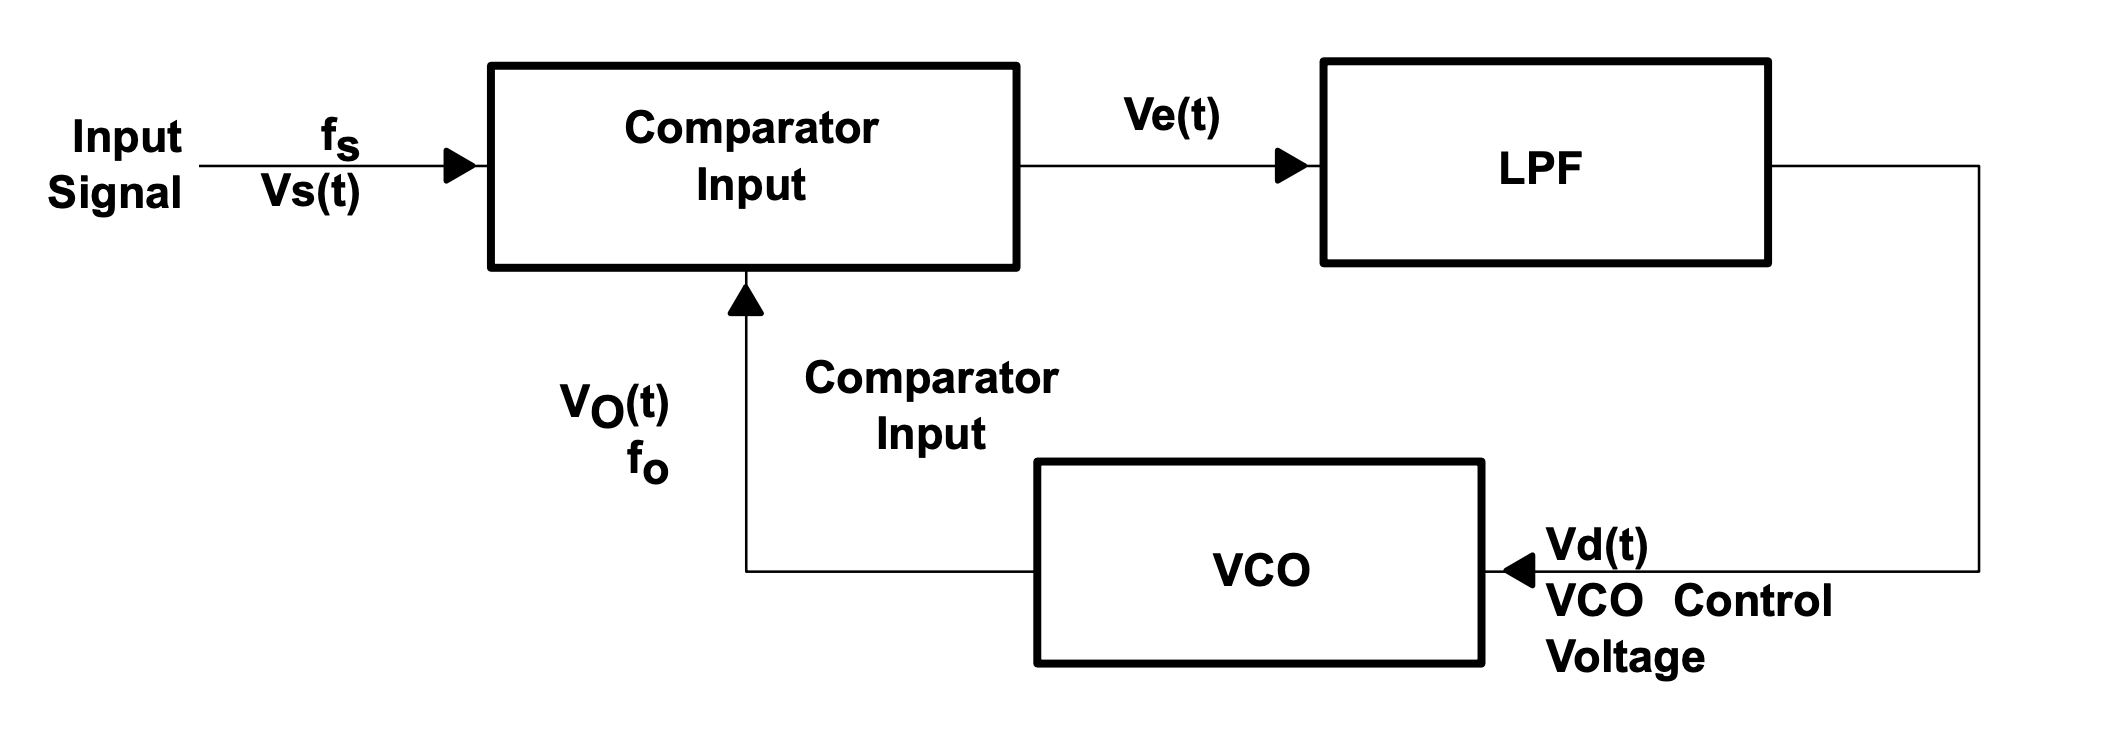
\includegraphics[width=0.8\textwidth]{resources/diagramabloquesPLL.png}
    \caption{Diagrama de bloques de un PLL básico}
    \label{diagramabloquesPLL}
\end{figure}
El producto de la multiplicación es filtrado por un filtro pasa-bajos de forma tal que se elimina el \emph{ripple} y el ruido de alta frecuencia, solo quedando en la salida una tensión proporcional a la diferencia de fase instantánea (la integral de la diferencia de frecuencia) entre las señales multiplicadas. Esta tensión controla la frecuencia del VCO. Si no hay señal en la entrada, no hay voltaje de error a la salida del comparador, por lo que tampoco lo hay a la salida del LPF. En esta situación, el VCO está fijo en su frecuencia central, $f_{0}$.

Como la entrada del control del VCO al variar reduce la diferencia de frecuencia entre el VCO y la señal de entrada y a su vez es proporcional a esta diferencia, la frecuencia del VCO tiende a la frecuencia de la señal de entrada, es decir, realiza un seguimiento de la misma. Cuando se llega a esta condición, se dice que el sistema está \emph{amarrado}.

Naturalmente, como consecuencia de la modulación, la frecuencia de la señal de entrada varía respecto de la frecuencia de la portadora, $f_{0}$. Existe un rango de frecuencias característico en el que es posible para el VCO realizar el seguimiento de frecuencias. Este rango se conoce como \emph{rango de enganche} y se discutirá más adelante.

Para aplicaciones en las que quiera detectarse un cambio de frecuencia en la señal de entrada, como en demoduladores de FM o FSK, se toma $v_{e}$ como salida del PLL. Si lo que se desea es "limpiar" una señal ruidosa, se toma como salida $\omega_{0}$: para una señal ruidosa, $v_{d}$ fluctúa alrededor de un valor medio. Si el filtro pasa-bajos es lo suficientemente preciso, $v_{e}$ será una señal limpia, dando lugar a una fase y frecuencia estables para el VCO.

\subsection{Rango de enganche}
Utilizando un comparador de fase cuya salida es proporcional al seno del ángulo de error de fase, la tensión de error $v_{e}$, tras pasar por el filtro pasa-bajos, será:
\begin{equation}\label{eqve}
    v_{e}(t)=K_{1}f(t)\ast sin[\phi_{i}(t)-\phi_{0}(t)]
\end{equation}
donde
\begin{equation*}
    K_{1}=AE/2
\end{equation*}
siendo E la amplitud de la señal de entrada y A la amplitud de la señal de la salida del VCO. $K_{1}$ aquí representa la ganancia de conversión del comparador de fase, y $f(t)$ es la respuesta al impulso del filtro pasa-bajos.
Asumiendo que la frecuencia del VCO es una función lineal de la tensión de error, esta será:
\begin{equation}
    \omega_{0}=\omega_{c}+\frac{d\phi_{0}}{dt}
\end{equation}
Reemplazando $\frac{d\phi_{0}}{dt}$ por $K_{2}v_{e}(t)$, donde $K_{2}$ tiene unidades de $\frac{rad}{V.s}$ y es la sensibilidad de tensión del VCO, y reemplazando $v_{e}$ según (\ref{eqve}), tenemos que:
\begin{equation}\label{eqdifvco}
    \frac{d\phi_{i}(t)}{dt}=\frac{d\phi}{dt}+Kf(t)\ast sin \phi(t)
\end{equation}
donde
\begin{equation*}
    K=K_{1}K_{2} rad/s
\end{equation*}
$\frac{d\phi_{i}(t)}{dt}$ representa la diferencia entre la frecuencia de la señal de entrada y la frecuencia de la portadora, $\Delta\omega_{i}$. Por lo tanto, asumiendo que la ganancia del filtro es 1, la solución de la ecuación \ref{eqdifvco} para estado estacionario es:
\begin{equation}\label{eqseno}
    sin\phi=\frac{\Delta\omega_{i}}{K}
\end{equation}
Se deduce que el sistema mantiene dicho estado, es decir, mantiene el enganche de frecuencias, siempre que:
\begin{equation}\label{leqq}
    |\Delta\omega_{i}| \leqq K
\end{equation}
La ecuación \ref{leqq} define el rango de enganche.
\subsection{Rango de captura}
El rango de captura es el rango de frecuencias dentro del cual la frecuencia del VCO puede sincronizarse con la frecuencia de la señal de entrada, partiendo de una situación de asincronismo. Si se tiene un filtro ideal que filtra solo las componentes de alta frecuencia y no atenúa las componentes de baja frecuencia de la señal, los rangos de captura y enganche coinciden. Si el filtro no es ideal y se quiere acotar el rango de enganche, reduciendo el ancho de banda del sistema, es muy probable que se vea restringido el rango de captura. Esto es un problema, ya que se dificulta el enganche fuera de condiciones iniciales. Con un rango de captura reducido, si se perturba el circuito y se produce un desenganche, no necesariamente se alcanzará nuevamente el sincronismo aunque la frecuencia de entrada se encuentre dentro del rango de enganche.

Si el sistema se encuentra en enganche, la transferencia del lazo no se ve afectada por el circuito pasa-bajos. Esta se ve gobernada por K, que define el rango de enganche, como se explicó en la sección anterior. Sin embargo, cuando el sistema no está enganchado, las frecuencias de las señales de entrada del comparador no son las mismas, y el VCO se ve controlado por una tensión de error variable, que puede ser atenuada por el filtro pasa-bajos. Esto es equivalente a modificar la ganancia del lazo, y es así como se genera la diferencia entre rango de captura y de enganche.

Si se expresa la transferencia del filtro pasa-bajos como
\begin{equation}
    F(j\omega)=F_{\omega}e^{j\psi(\omega)}
\end{equation}
se tiene que la tensión de error es
\begin{equation}
    v_{e}(t)=K_{1}F_{\Delta\omega_{i}} sin \Delta\omega_{i}t
\end{equation}
Para la frecuencia de captura $\omega_{ic}$, el valor pico de la tensión de error es
\begin{equation}\label{eqvec}
    \hat{v_{ec}}=K_{1}F_{\Delta\omega_{ic}}
\end{equation}
Por definición, al alcanzar la frecuencia de captura, el circuito entra en estado estacionario. La tensión de error para estado estacionario es
\begin{equation}\label{eqvec2}
    v_{ec}=K_{1} sin\psi_{c}
\end{equation}
Igualando las expresiones \ref{eqvec} y \ref{eqvec2} y reemplazando con la expresión \ref{eqseno}, tenemos que
\begin{equation}
    v_{ec}=K_{1}(\frac{\Delta\omega_{i}}{K})
\end{equation}
entonces, el rango de captura es 
\begin{align}\label{rangocap}
    (\omega_{i}-\omega_{c} &, \omega_{i}+\omega_{c})   &   \omega_{c}&=KF_{\Delta\omega_{ic}}
\end{align}
\subsubsection{Efectos de distintos filtros sobre el rango de captura}
Para un filtro pasa-bajos de transferencia $F_{\omega}=1$, el rango de captura es igual al de enganche, por razones expuestas anteriormente.
\begin{figure}[H]
        \centering
        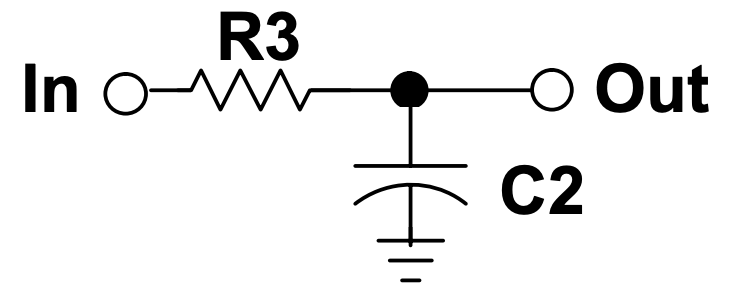
\includegraphics[width=0.4\textwidth]{resources/filtrorc.png}
        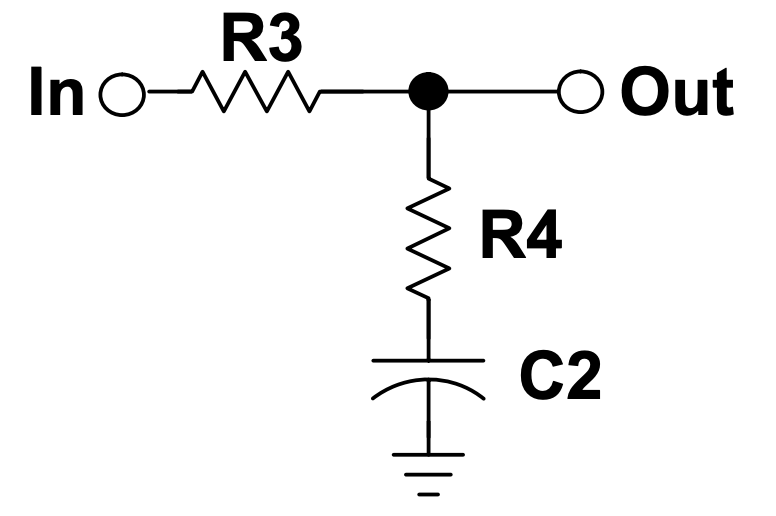
\includegraphics[width=0.4\textwidth]{resources/filtrorrc.png} 
    \caption{Filtros normalmente utilizados en diseño de PLL}
\end{figure}
Para un filtro pasa-bajos de orden 1, cuya transferencia es 
\begin{equation}
    F_{\omega}=\frac{1}{(1+\omega^2(RC)^2)^{1/2}}
\end{equation}
el rango de captura, según \ref{rangocap}, es
\begin{equation}
    \frac{\Delta\omega_{ic}}{K}=\left[\frac{\omega_{co}}{K}\left(1+\frac{1}{4}\left(\frac{\omega_{co}}{K}\right)^2\right)^{\frac{1}{2}}-\frac{1}{2}\left(\frac{\omega_{co}}{K}\right)^2\right]^\frac{1}{2}
\end{equation}
Este resultado se ve graficado en función del ancho de banda del filtro en la Figura \ref{engancheprimerorden}.

\begin{figure}[H]
    \centering
    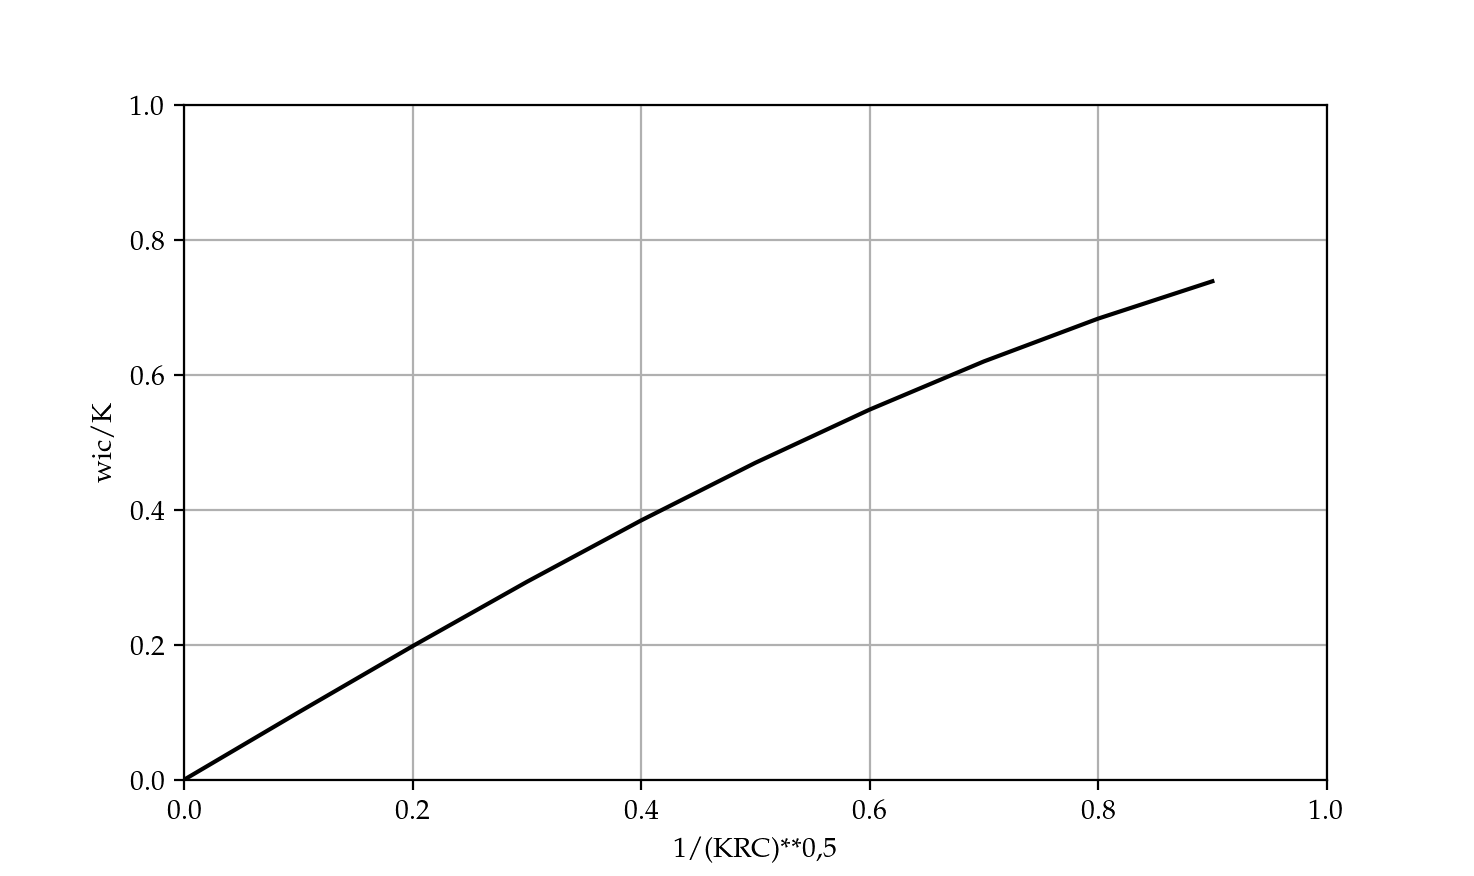
\includegraphics[width=0.8\textwidth]{resources/engancheprimerorden.png}
    \caption{Relacion rango captura/rango enganche del VCO en función del ancho de banda del filtro pasa-bajos de primer orden}
    \label{engancheprimerorden}
\end{figure}
Se observa que a menor ancho de banda del filtro, menor es la relación entre el rango de captura y el rango de enganche del VCO.

Para un filtro del tipo RRC, cuya transferencia es

\begin{equation}
    F_{\omega}=\left[\frac{1+\omega^2\tau_{1}^2}{1+\omega^2\tau_{2}^2}\right]^{\frac{1}{2}}
\end{equation}
donde
\begin{align*}   
    \tau_{1}&=R_{4}C_{2} & \tau_{2}&=(R_{4}+R_{3})C_{2}
\end{align*}
reemplazando las siguientes expresiones,
\begin{align}\label{zetatau}
    2\zeta \frac{\omega_{n}}{K}
    &=\frac{1+K\tau_{1}}{K\tau_{2}} & \left(\frac{\omega_{n}}{K}\right)^2&=\frac{1}{K\tau_{2}}
\end{align}
se obtiene la siguiente relación:
\begin{equation}\label{eqdifsegundoorden}
    \frac{\Delta\omega_{ic}}{K}=\frac{\omega_{n}}{K}\left[\left(\left[2\zeta\left(\frac{\omega_{n}}{K}\right)\right]^2+1\right)^\frac{1}{2}-2\zeta\left(\frac{\omega_{n}}{K}-\zeta\right)\right]^\frac{1}{2}
\end{equation}
La ecuación \ref{eqdifsegundoorden} representa la relación rango de captura - rango de enganche en función del \emph{damping} del filtro RRC. $\omega_{n}$ representa la frecuencia natural del sistema, mientras que $\zeta$ es la relación entre el \emph{damping} real y crítico de la transferencia de lazo cerrado del PLL. Esta relación se puede observar para distintos valores de $\frac{\omega_{n}}{K}$ en la Figura \ref{enganchesegundoorden}.

\begin{figure}[H]
    \centering
    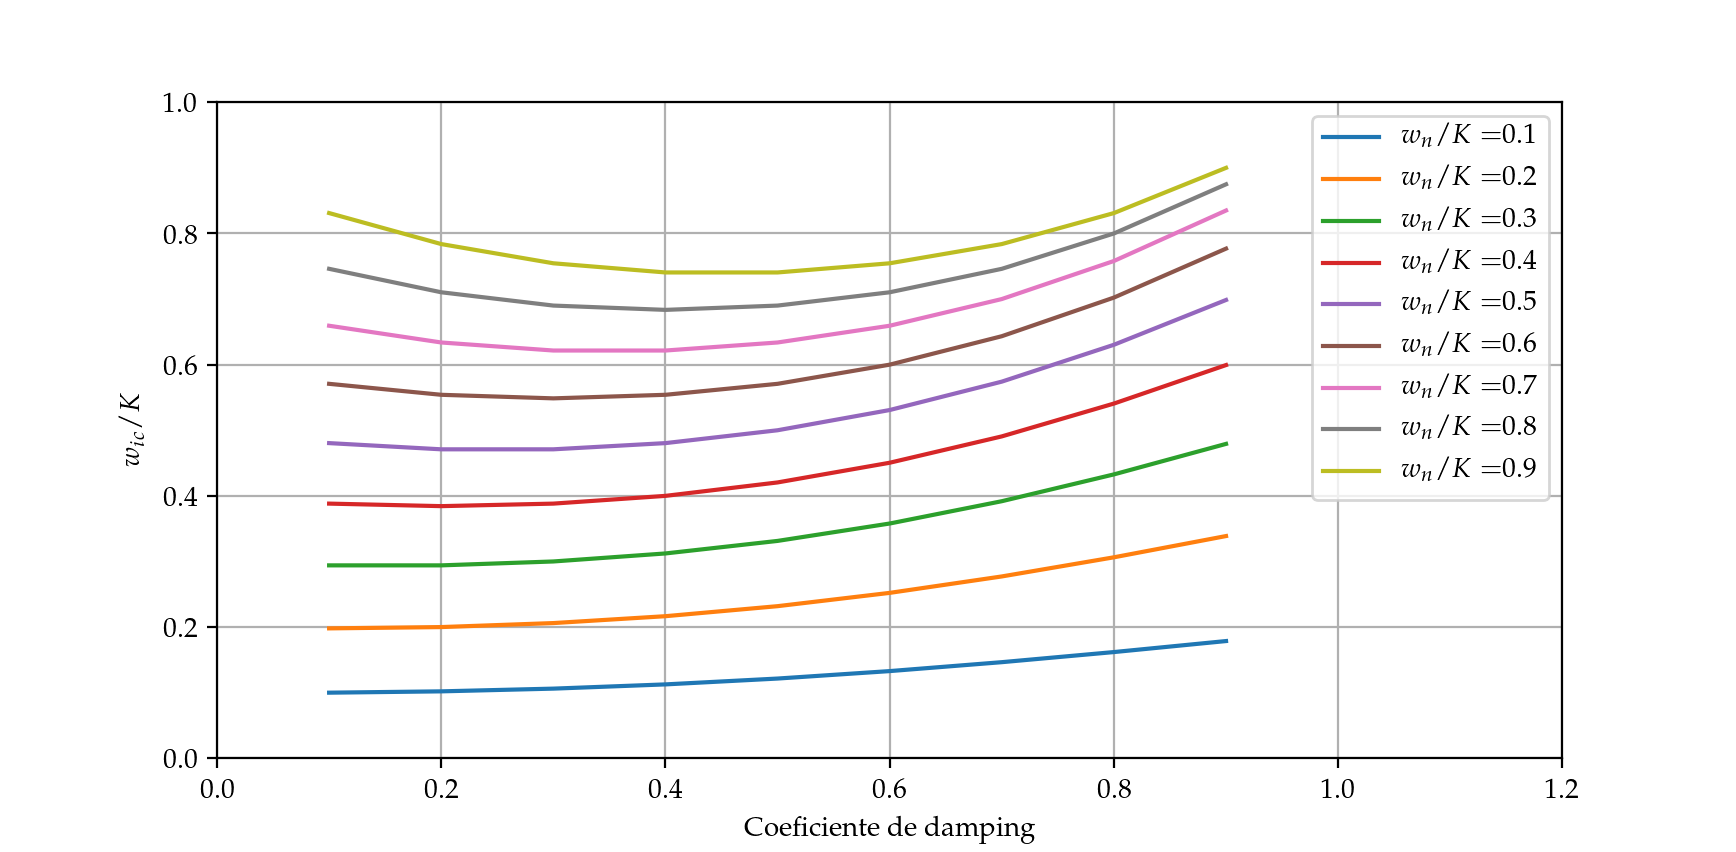
\includegraphics[width=\textwidth]{resources/enganchesegundoorden.png}
    \caption{Relacion rango captura/rango enganche del VCO en función del ancho de banda del filtro RRC para distintos valores de $\frac{\omega_{n}}{K}$}
    \label{enganchesegundoorden}
\end{figure}

Se sabe que $\zeta=\frac{1}{2Q}$, donde Q es el factor de calidad del filtro. La ventaja que tiene usar un filtro RRC es que, como se observa en la Figura \ref{enganchesegundoorden}, se puede seleccionar $\omega_{n}$ modificando el valor de $\tau_{2}$ del filtro pasa-bajos (\emph{ver ecuación \ref{zetatau}}) para mantener el rango de captura muy cercano al de enganche para cualquier sensibilidad.


\section{Composición del integrado CD4046B}
El integrado \emph{CD4046B}, utilizado en el presente informe, se compone de un VCO y dos comparadores de fase para escoger, de los cuales se utiliza solo uno a la vez. El esquemático de este integrado se muestra en la Figura \ref{integradoadentro}.
\begin{figure}[H]
    \centering
    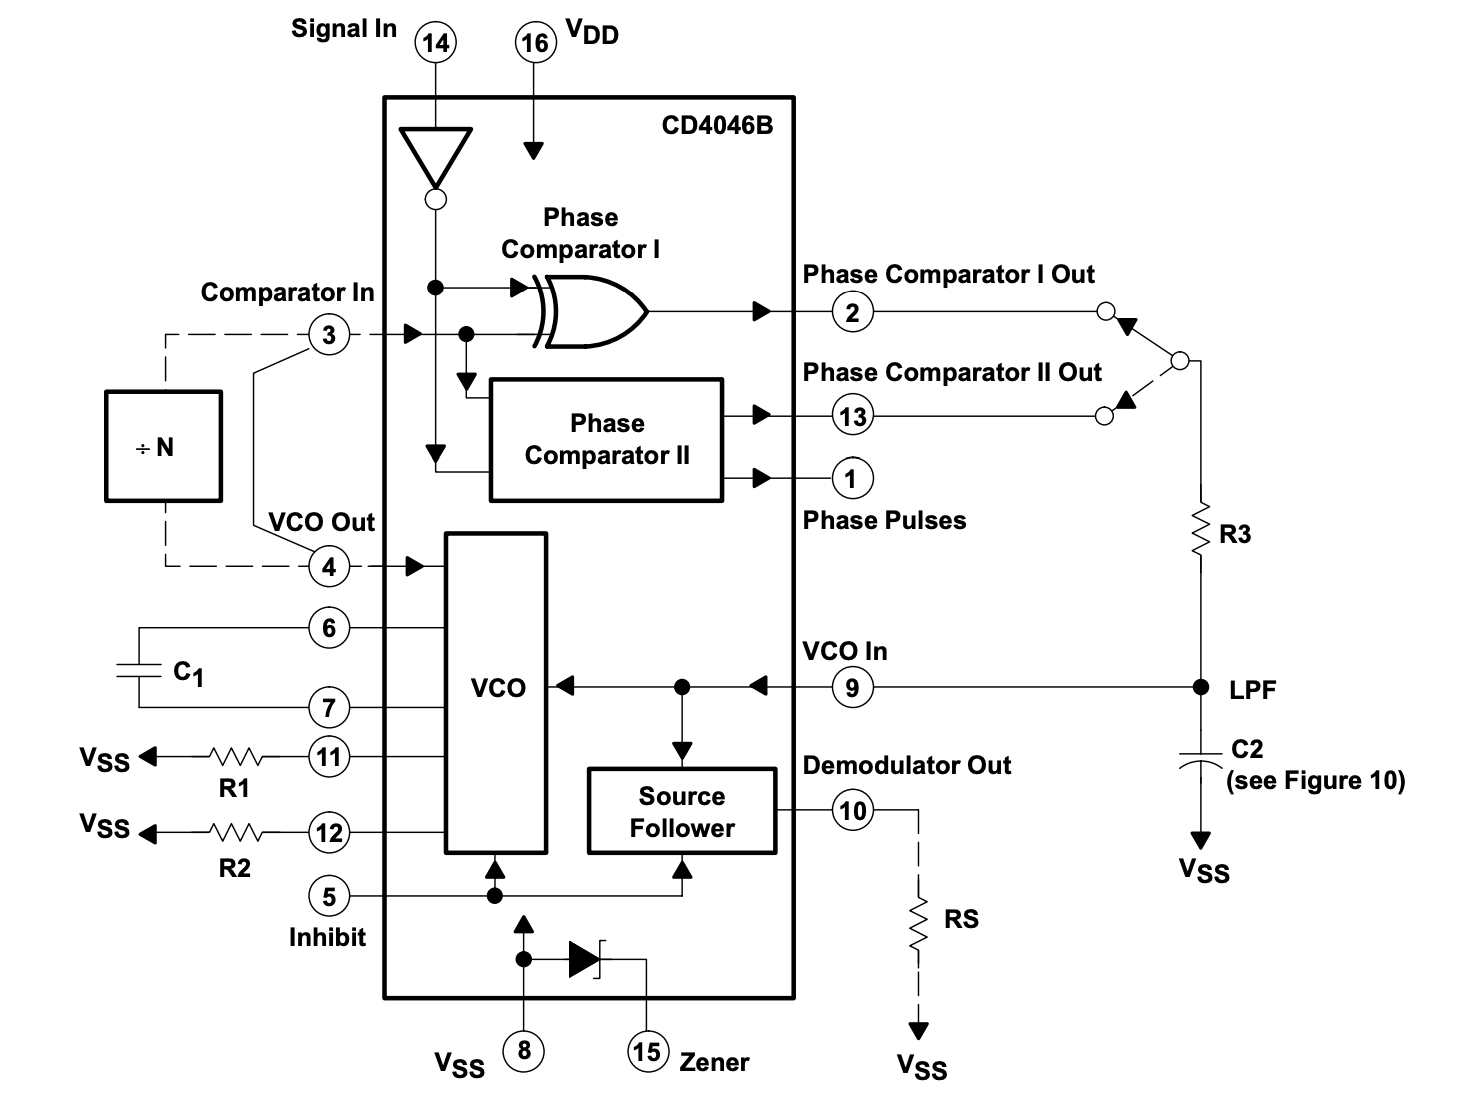
\includegraphics[width=0.8\textwidth]{resources/integradoadentro.png}
    \caption{Esquemático del integrado CD4046B}
    \label{integradoadentro}
\end{figure}

\subsection{Comparadores de fase}
El esquemático de la etapa de comparadores del circuito se observa en la Figura \ref{comparadoresfasePLL}. 
\begin{figure}[H]
    \centering
    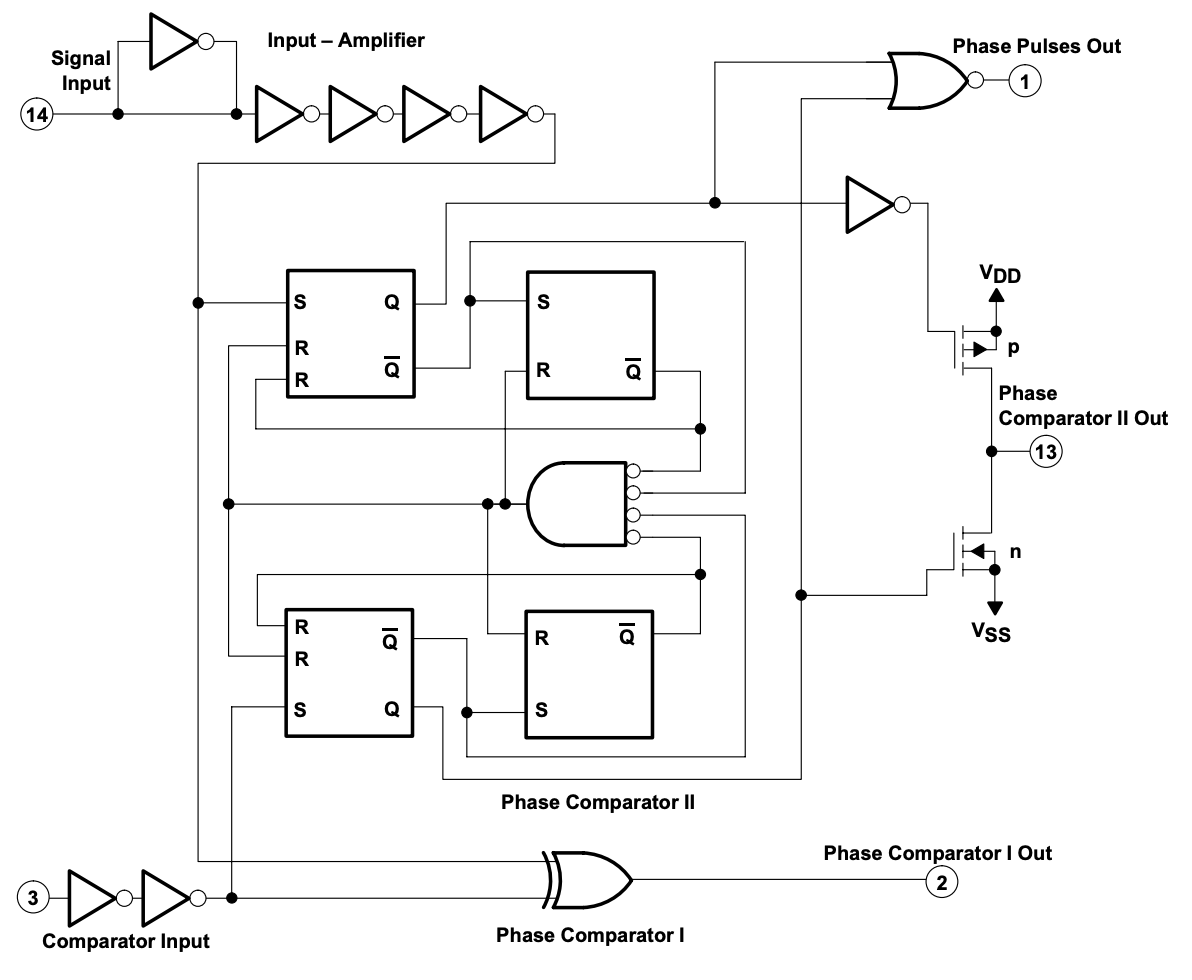
\includegraphics[width=0.8\textwidth]{resources/comparadoresfasePLL.png}
    \caption{Etapa de comparadores del integrado CD4046B}
    \label{comparadoresfasePLL}
\end{figure}
Se observa que el comparador I es una compuerta XOR, de modo que la señal a la salida está en estado activo cuando las señales a la entrada están en estados distintos. El \emph{duty cycle} de esta señal es función de la diferencia entre las señales de entrada. 

Al pasar por el filtro pasa-bajos, la señal cuadrada de \emph{duty cycle} variable se transformará en otra, cuya tensión es función del valor medio de la anterior, es decir aumenta cuando hay diferencia en las señales y disminuye cuando no la hay. Es esta la señal que controla el VCO. Esto puede verse en la Figura \ref{ondascomparador1PLL}.

\begin{figure}[H]
    \centering
    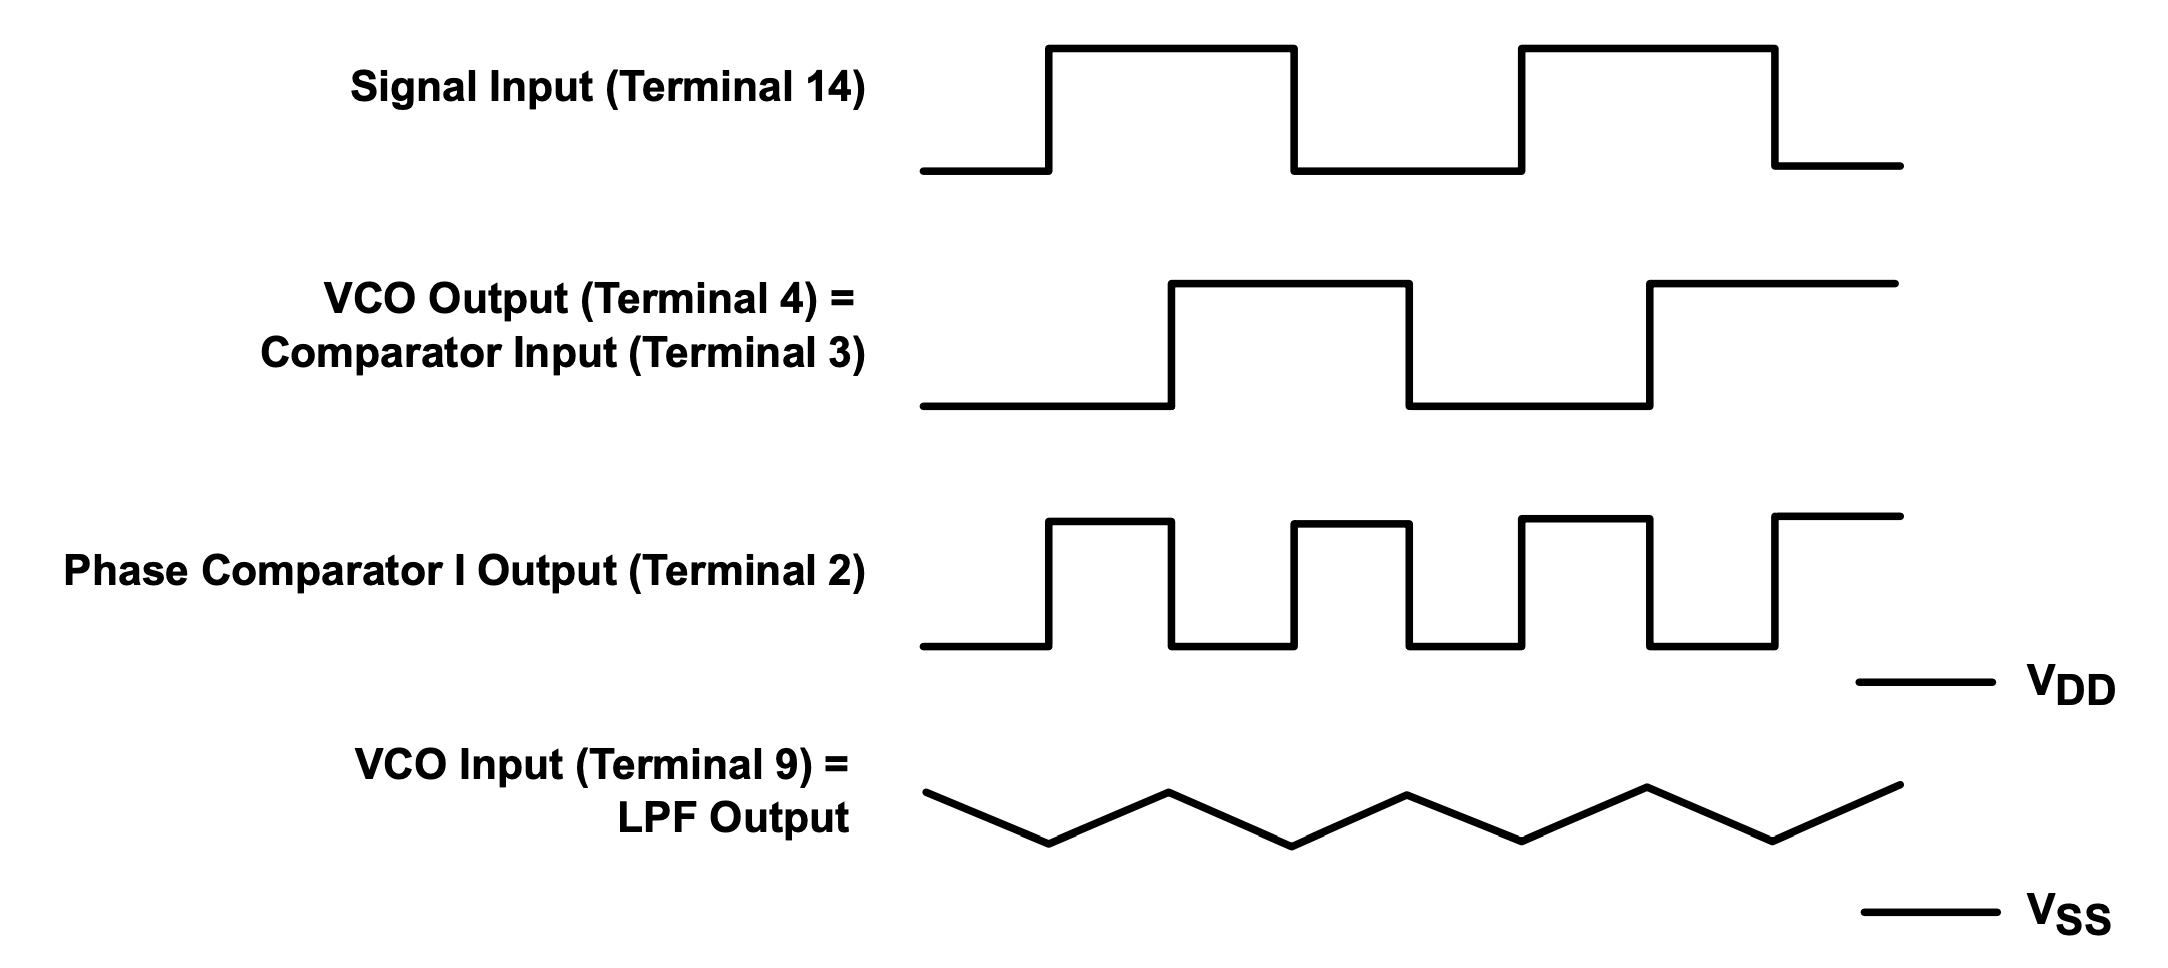
\includegraphics[width=0.8\textwidth]{resources/ondascomparador1PLL.png}
    \caption{Ondas del PLL con comparador 1}
    \label{ondascomparador1PLL}
\end{figure}

Hace falta tener en cuenta dos particularidades: que este comparador puede hacer tender el sistema a frecuencias de entrada cercanas a armómicos de la frecuencia central del VCO, $f_{0}$, y que la diferencia de fase que admite en sus entradas varía entre 0 y 180 grados, y es de 90 para la frecuencia $f_{0}$. La relación diferencia de fase - tensión de salida del LPF para este comparador se muestra en la Figura \ref{relacionfasevoltajecomp1PLL}.

\begin{figure}[H]
    \centering
    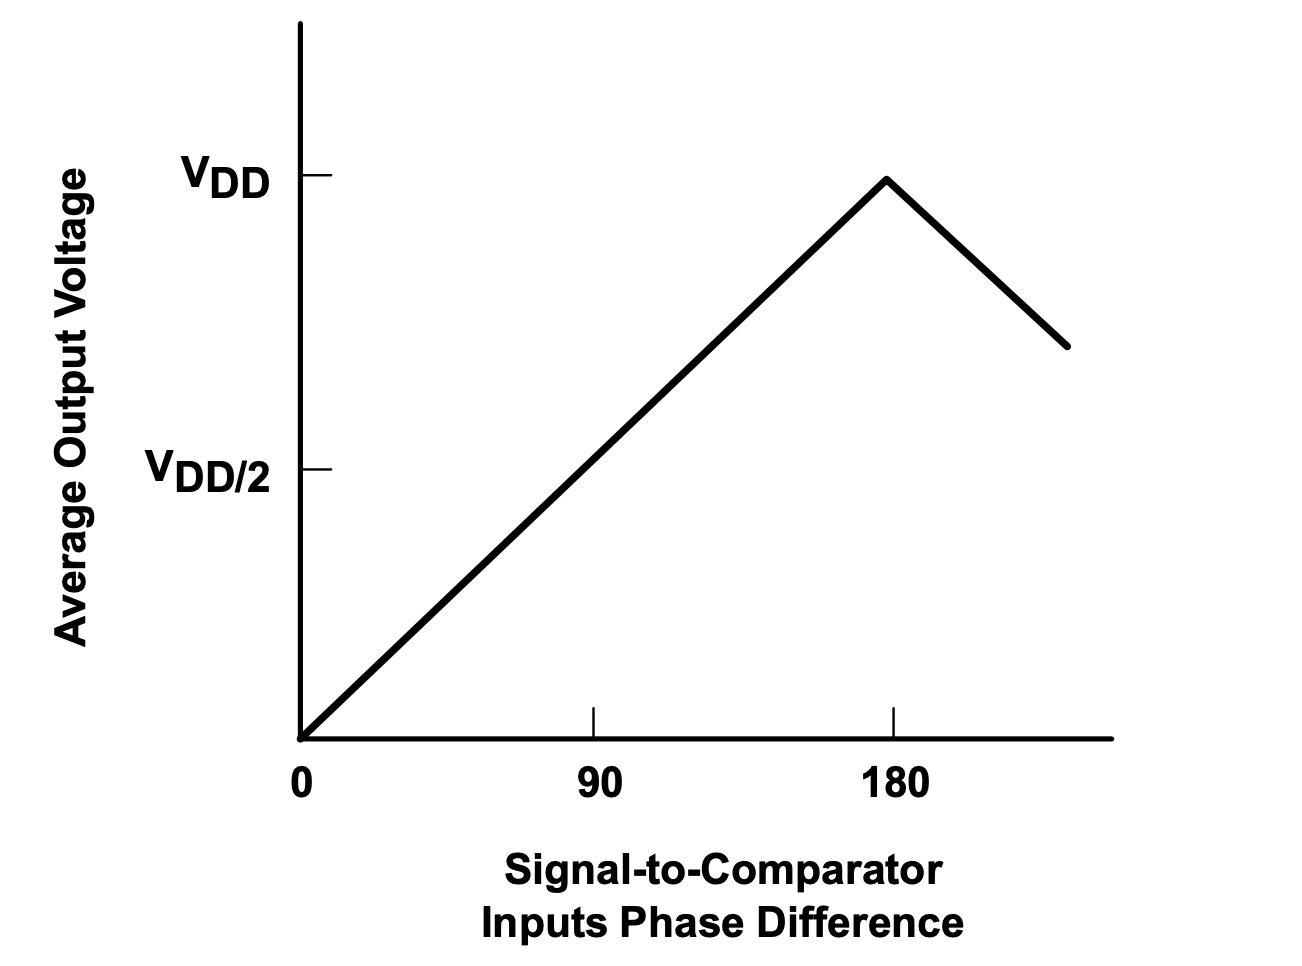
\includegraphics[width=0.6\textwidth]{resources/relacionfasevoltajecomp1PLL.png}
    \caption{Relación diferencia de fase en comparador - tensión a la salida del LPF}
    \label{relacionfasevoltajecomp1PLL}
\end{figure}

El comparador 2 es algo más complejo y no será desarrollado, puesto que el comparador a utilizar a los propósitos del presente informe es el primero.

\subsection{Oscilador controlado por voltaje (VCO)}
El oscilador interno del integrado permite regular su frecuencia central, $f_{0}$, mediante la selección de los componentes C1 y R1, que se conectan externamente. La relación de la frecuencia central con C1 para varios valores de R1 se muestra en la Figura \ref{f0vsc1r1pll}.

\begin{figure}[H]
    \centering
    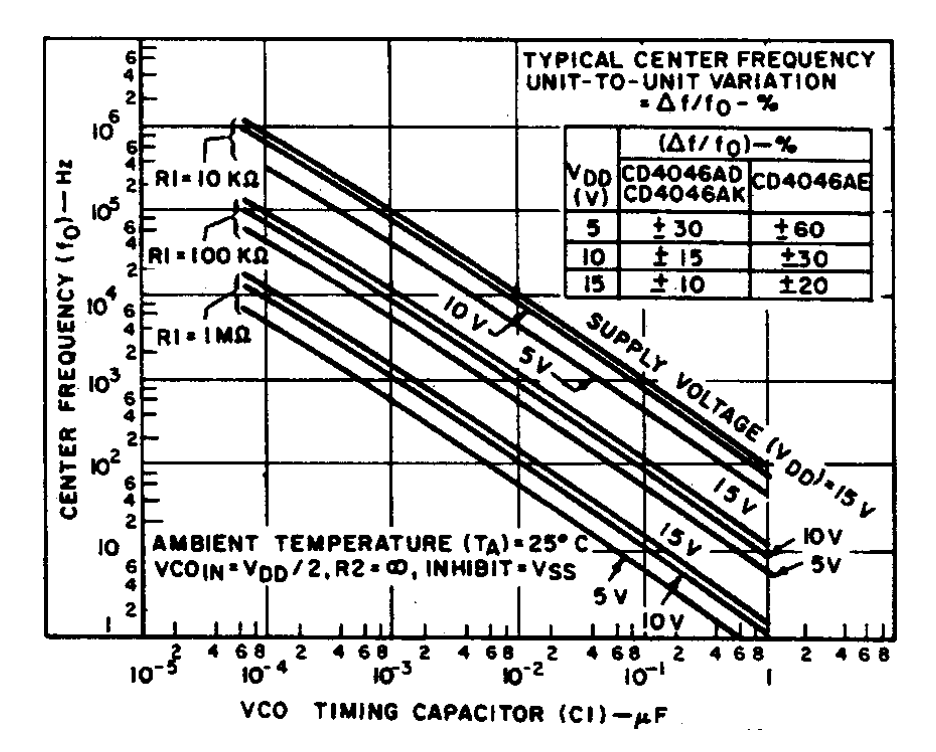
\includegraphics[width=0.5\textwidth]{resources/f0vsc1r1pll.png}
    \caption{Relación de $f_{0}$ con C1 para varios valores de R1}
    \label{f0vsc1r1pll}
\end{figure}

\section{Implementación del integrado}
Se implementó el integrado para diseñar un PLL con un rango de enganche que abarca desde $6kHz$ hasta $98kHz$.

Se seleccionó una frecuencia central $f_{o}=50kHz$. Con una alimentación de 5V, según la Figura \ref{f0vsc1r1pll}, para que oscile a esa frecuencia los valores de C1 y R1 deben ser de aproximadamente $70pF$ y $10k\Omega$, respectivamente.

Se implementaron en el PCB mediante un \emph{jumper} tres opciones distintas en el lugar para la etapa de filtrado de la señal: una opción para saltar la etapa, un filtro RC y un filtro RRC.

\subsection{Medición del factor de calidad Q}
Para obtener el valor de Q, se midió la respuesta al escalón del PLL en la entrada de control del VCO. Se define:
\begin{equation}
    Q=\frac{1}{2\zeta}
\end{equation}
\begin{equation}
    \zeta=\frac{-ln(OS)}{\sqrt{\pi^2+ln^2(OS)}}
\end{equation}
\begin{equation}
    OS=\frac{V_{pico}-V_{estacionario}}{V_{estacionario}}
\end{equation}
En las figuras \ref{escalonrc} y \ref{escalonrrc} se pueden ver las mediciones de la respuesta al escalón de frecuencia mencionado anteriormente, y en la Tabla \ref{tablarespesc} se muestra la información reunida de dicho experimento.
\begin{figure}[H]
    \centering
    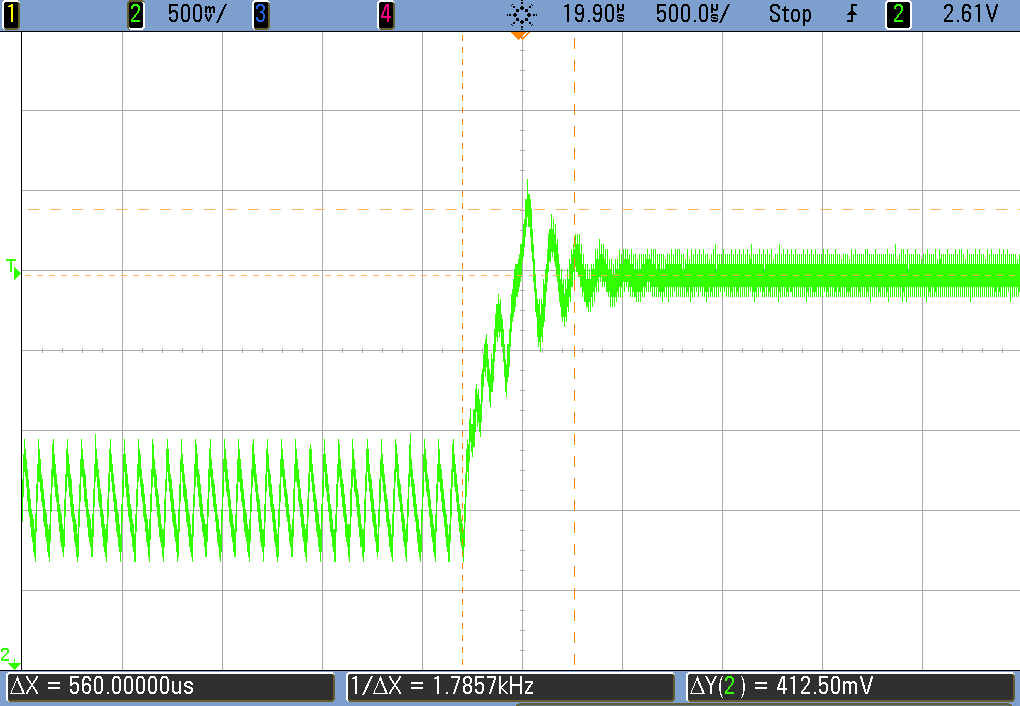
\includegraphics[width=0.9\textwidth]{resources/escalonrc.png}
    \caption{Medición: respuesta del PLL al escalón de frecuencia (sin filtro)}
    \label{escalonrc}
\end{figure}

\begin{figure}[H]
    \centering
    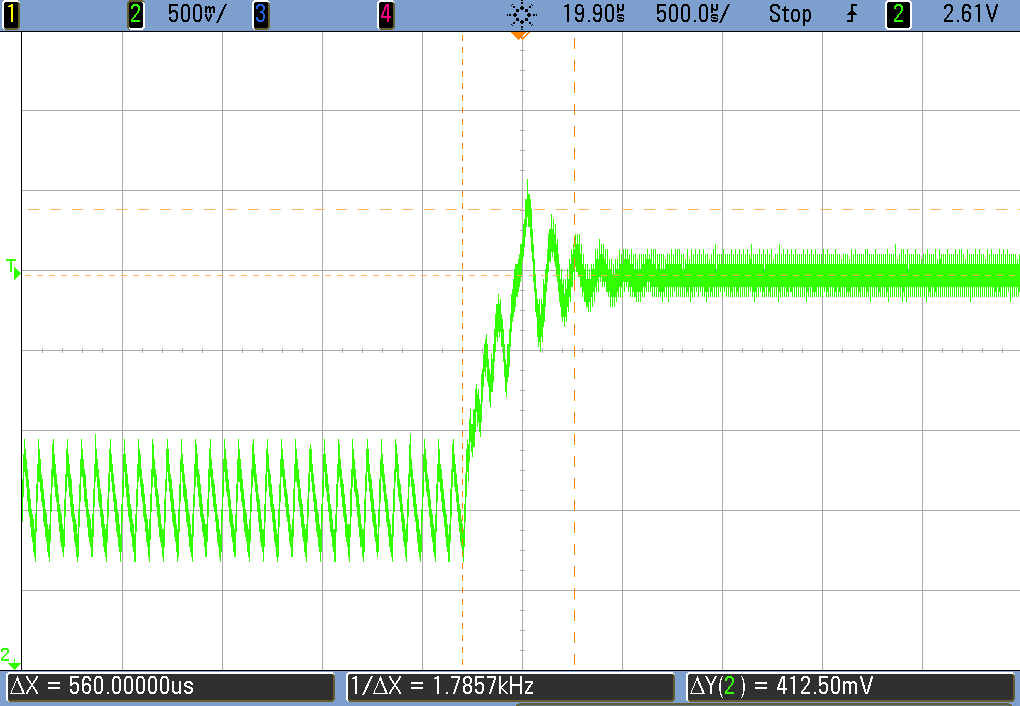
\includegraphics[width=0.9\textwidth]{resources/escalonrc.png}
    \caption{Medición: respuesta del PLL al escalón de frecuencia (filtro RC)}
    \label{escalonrc}
\end{figure}

\begin{figure}[H]
    \centering
    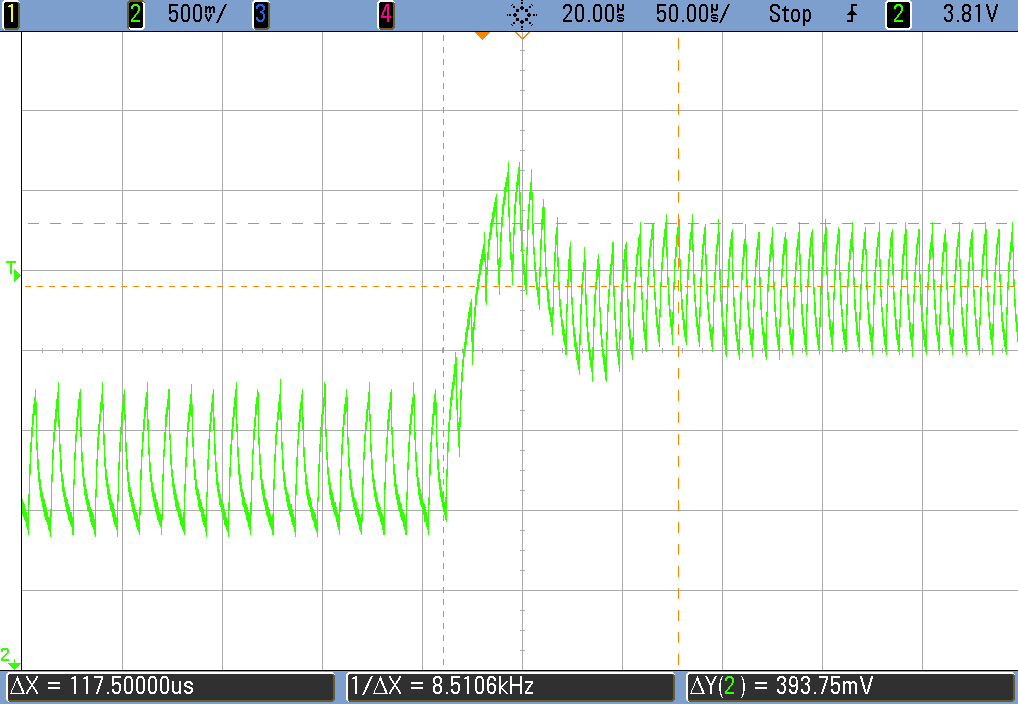
\includegraphics[width=0.9\textwidth]{resources/escalonrrc.png}
    \caption{Medición: respuesta del PLL al escalón de frecuencia (filtro RRC)}
    \label{escalonrrc}
\end{figure}

\begin{table}[H]
    \centering
    \begin{tabular}{|c|c|c|c|c|}
    \hline
                &  OS   &   \zeta  & Q    &   T_{est}   \tabularnewline
    \hline
    \hline
    Sin Filtro &          &       &        &            \tabularnewline
    \hline
    Filtro RC  &         &         &        &            \tabularnewline 
    \hline
    Filtro RRC &         &       &         &           \tabularnewline
    \hline
    \end{tabular}
    \caption{Mediciones de parámetros del transitorio}
    \label{tablacaptura}
\end{table}

Se observa que
%TODO: medir la respuesta al escalón para los dos filtros. seguramente, las oscilaciones tengan el mismo pseudoperiodo. incluirlo. 
%tomar nota también del tiempo de establecimiento, es decir el tiempo desde el pico hasta el estado estacionario. va a ser menor para el filtro rrc porque es más cheto


\subsection{Medición del tiempo de enganche y captura}
Se realizaron mediciones del rango de enganche y captura. 

La Figura \ref{varfrecvarve} muestra la variación de la tensión de entrada del VCO respecto de la variación de frecuencia para los distintos filtros. Los resultados obtenidos de estos gráficos se pueden observar en la Tabla \ref{tablacaptura}.

\begin{figure}[H]
    \centering
    \includegraphics[width=0.9\textwidth]{resources/varfrecvarve.png}
    \caption{Variación de $v_{e}$ con la frecuencia de entrada para un rango de 0 a 100kHz}
    \label{varfrecvarve}
\end{figure}

Se observa que %TODO: medir con el bodeador, en tres experiencias (una por filtro) de dos etapas cada una (aumentando y disminuyendo la frecuencia), la tensión de entrada del vco mientras se varía la frecuencia de la señal de entrada. El bodeador guarda los valores de tensión en la planilla que exporta. graficar tensión en la entrada del vco versus frecuencia de la señal de entrada. para cada experimento, superponer las curvas.
%cuando acopla, estamos en frecuencia de captura. cuando desacopla, frecuencia de enganche

\begin{table}[H]
    \centering
    \begin{tabular}{|c|c|c|c|}
    \hline
                &Intervalo Captura  &   Intervalo Enganche  & $f_{0}$   \tabularnewline
    \hline
    \hline
    Sin Filtro &                   &                       &           \tabularnewline
    \hline
    Filtro RC  &                   &                       &           \tabularnewline 
    \hline
    Filtro RRC &                   &                       &           \tabularnewline
    \hline
    \end{tabular}
    \caption{Mediciones de rango de enganche y captura}
    \label{tablacaptura}
\end{table}



\subsection{Aplicación: demodulación FM}
\subsubsection{Introducción: modulación FM}
El principio básico tras el concepto de modulación en frecuencia (FM, por sus siglas en inglés) es que la amplitud de una señal analógica, a la que llamaremos la señal modulada, puede ser representada por un cambio en la frecuencia de otra, a la que llamaremos la señal portadora. De esta forma, distintas amplitudes de la primera corresponden a frecuencias específicas de la segunda. Esto se ve ilustrado en la Figura \ref{modulacionfmsenales}
\begin{figure}[H]
    \centering
    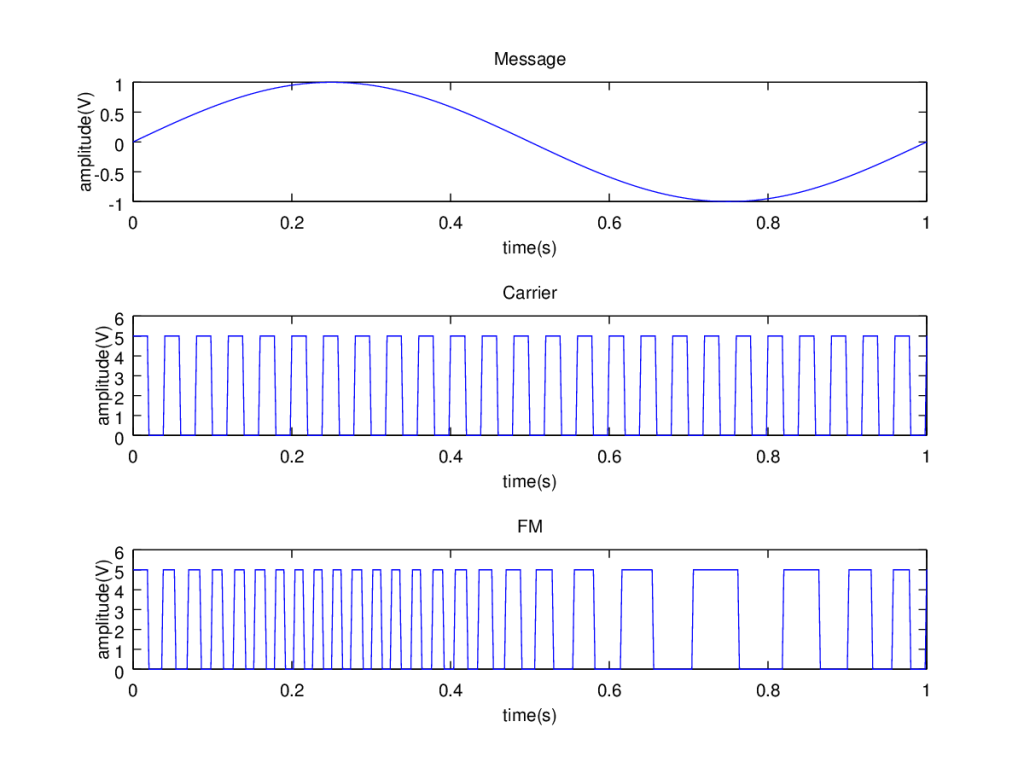
\includegraphics[width=0.9\textwidth]{resources/modulacionfmsenales.png}
    \caption{Modulación FM: portadora, modulada y FM}
    \label{modulacionfmsenales}
\end{figure}

\subsubsection{Implementación}
Se implementó el integrado en un circuito para demodular una señal FM con portadora de $50kHz$ modulada por una señal de audio de frecuencia $f_{1}=400Hz$. A continuación, se detalla su funcionamiento.
\begin{figure}[H]
    \centering
    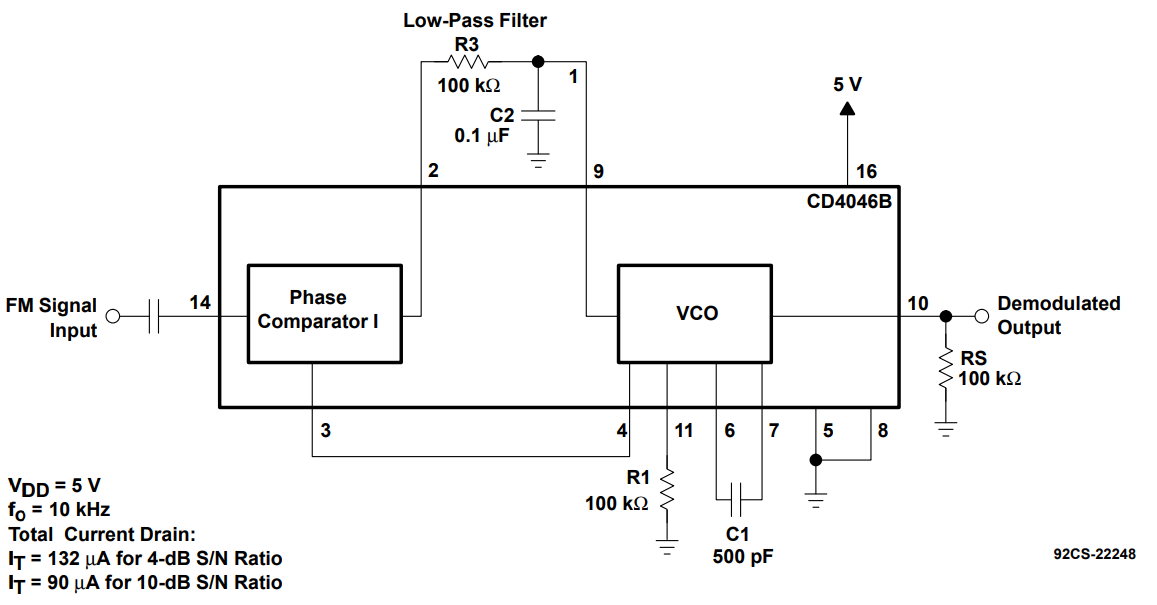
\includegraphics[width=0.9\textwidth]{resources/demoduladorfmconexion.png}
    \caption{Esquemático del circuito del demodulador FM}
    \label{demoduladorfmconexion}
\end{figure}

Cuando se pone en la entrada de un PLL una señal FM y se produce el enganche de frecuencias, se realiza un seguimiento de su frecuencia. La amplitud de la señal de entrada del VCO en esta situación, es decir la tensión de error del comparador de fase tras pasar por el filtro, es proporcional a la diferencia entre la frecuencia del VCO y la frecuencia de la señal FM. Si se configura el VCO con una $f_{0}$ igual a la de la portadora de la señal FM, esta señal corresponde a la señal FM demodulada, es decir, la señal modulada original.

Con esta configuración, según la Figura \ref{f0vsc1r1pll}, la frecuencia central del VCO será de aproximadamente $50kHz$. Se coloca un capacitor de desacople en la entrada para eliminar el nivel de contínua de la señal FM. A su vez, el rango de captura de esta configuración es de $f_{c}=\pm \frac{f_{1}}{R_{3}C_{2}}=\pm0,4kHz$, donde $f_{1}$ es la frecuencia de la señal modulada y  $R_{3}$ y $C_{2}$ son los valores de los componentes del filtro pasa-bajos. Con este rango de captura, se permite realizar la captura de la señal aunque su frecuencia no sea exactamente la de la portadora, por efectos de la modulación.

El pin 10 del integrado, que corresponde a la salida de la señal demodulada, está internamente conectado mediante un \emph{buffer} a la entrada del VCO, es decir, la salida del filtro pasa-bajos.

Esta configuración solo demodula la señal especificada, pero bastaría con modificar los valores de los componentes $R_{1}$ o $C_{1}$ para variar la frecuencia a seguir, o los valores de $R_{3}$ y $C_{2}$ para modificar el rango de captura. Reemplazando $R_{1}$ por un potenciómetro adecuado, podría incluso implementarse un demodulador FM de frecuencia variable.

\subsubsection{Mediciones}
Se utilizaron generadores de señal para modular en frecuencia con varias señales de audio de 400Hz una portadora de 10kHz. Las señales FM resultantes se transmitieron al PLL implementado en PCB para ser demodulado.

Se muestran en las figuras \ref{demodulacionfmcuadrada}, \ref{demodulacionfmsenoidal} y \ref{demodulacionfmrampa} las mediciones de la señal moduladora, la FM y la demodulada para moduladoras de forma cuadrada, senoidal y de rampa, respectivamente. 
\begin{figure}[H]
    \centering
    \includegraphics[width=0.9\textwidth]{resources/demodulacionfmcuadrada.png}
    \caption{Medición: demodulación de señal cuadrada}
    \label{demodulacionfmcuadrada}
\end{figure}
\begin{figure}[H]
    \centering
    \includegraphics[width=0.9\textwidth]{resources/demodulacionfmsenoidal.png}
    \caption{Medición: demodulación de señal senoidal}
    \label{demodulacionfmsenoidal}
\end{figure}
\begin{figure}[H]
    \centering
    \includegraphics[width=0.9\textwidth]{resources/demodulacionfmrampa.png}
    \caption{Medición: demodulación de señal rampa}
    \label{demodulacionfmrampa}
\end{figure}
Se puede ver que %TODO: modular la señal a lo labo de electronica con los dos generadores, metérsela y ver qué sale. medir todo lo que menciona el informe, graficarlo junto y ponerlo acá. sacar conclusiones a partir de las diferencias entre la moduladora y la demodulada.

\subsection{Implementación: multiplicador de frecuencias}
Se implementó el PLL como un multiplicador de frecuencias mediante la conexión de un contador de décadas que actúa de divisor de frecuencias entre la salida del VCO y la entrada del comparador. De esta manera, el PLL realiza un seguimiento de  % TODO: implementar circuito con CD4016

La salida del PLL será una señal de frecuencia $Nf_{in}$, donde N es un entero función del divisor de frecuencias y varía entre 1 y 10, y $f_{in}$ es la frecuencia de la señal de entrada del PLL.

Se utilizó para esta aplicación el comparador de fase II, ya que no tiende a seguir a los armónicos de la señal de entrada, lo cual es relevante ya que el \emph{duty cycle} de la salida del divisor no es del 50\%.

Se utilizó también un filtro RRC para esta aplicación, ya que tiene un tiempo de establecimiento más corto y permite rápida adaptación a los saltos de frecuencia introducidos por el selector de frecuencia del divisor. % TODO: relacionar esto a resp escalon

\subsubsection{Mediciones}
En las figuras \ref{medicionstep2}, \ref{medicionstep4} y \ref{medicionstep8} se observan las mediciones de la señal de entrada y salida del PLL para las configuraciones N=2, N=4 y N=8, respectivamente.

\section{Conclusión}
El PLL es un circuito versátil, que puede ser implementado para demodular señales FM y FSK, multiplicar frecuencias, sincronizar \emph{clocks} y sintetizar frecuencias, entre otras aplicaciones.

Mediante la selección de componentes adecuados en el diseño, se puede escoger de un amplio rango de valores de operación, además de optimizar el diseño para distintas aplicaciones que exijan tiempos de establecimiento y selectividad de frecuencias específicas.

\section{Referencias}
Phase-Locked Loop Design Fundamentals: \url{https://www.nxp.com/files-static/rf_if/doc/app_note/AN535.pdf}

CD4046B Phase-Locked Loop: A Versatile Building
Block for Micropower Digital and Analog Applications: \url{http://www.ti.com/lit/an/scha002a/scha002a.pdf}

Miniaturized RC Filters Using Phase-Locked Loop. (Moschytz, G.S.): \url{https://ia801902.us.archive.org/17/items/bstj44-5-823/bstj44-5-823.pdf}

CMOS Phase-Locked-Loop Applications Using the
CD54/74HC/HCT4046A and CD54/74HC/HCT7046A: \url{http://www.ti.com/lit/an/scha003b/scha003b.pdf}

\end{document}

